\section{Methodology}

The methodology of this study is designed to ensure that each technical indicator is rigorously defined, mathematically formulated, and consistently applied across all selected markets and asset classes. By adopting a unified computational framework, the analysis maintains comparability between Indian, UK, and US funds, even when their volatility profiles and market structures differ. 

Each indicator is presented with its theoretical foundation, calculation process, and interpretive framework, followed by its role within the overall trading strategy. This structured approach not only facilitates transparency in implementation but also enables robust statistical evaluation of cross-market performance.


\subsection{Technical Indicators}


\subsubsection{Bollinger Bands}
Bollinger Bands, developed by John Bollinger in the early 1980s, are one of the most widely adopted technical indicators for assessing volatility and relative price levels in financial markets. They are constructed using a moving average and standard deviation measures to create a dynamic envelope around price. This approach allows the bands to expand and contract in response to market volatility, making them adaptable to different asset classes, markets, and timeframes. In the context of cross-market analysis, such as Indian, UK, and US funds, Bollinger Bands provide a consistent framework for comparing price behaviour across diverse volatility regimes.

Mathematically, Bollinger Bands consist of three key components: the Middle Band (a moving average), the Upper Band (Middle Band plus a multiple of standard deviation), and the Lower Band (Middle Band minus the same multiple of standard deviation). Let $P_t$ denote the closing price of an asset at time $t$, and let $n$ be the look-back period, typically set to 20 for daily data. The Middle Band is calculated as:
\[
MB_t = \frac{1}{n} \sum_{i=0}^{n-1} P_{t-i}
\]
This moving average provides the central tendency of recent prices and serves as a reference point for measuring deviations.

The standard deviation over the same $n$ periods is defined as:
\[
\sigma_t = \sqrt{\frac{\sum_{i=0}^{n-1} \left(P_{t-i} - MB_t \right)^2}{n}}
\]
In some statistical contexts, the denominator $n-1$ is used to produce the sample standard deviation; however, in most financial implementations, $n$ is used for computational simplicity and consistency.

The Upper and Lower Bands are then computed as:
\[
UB_t = MB_t + k \cdot \sigma_t
\]
\[
LB_t = MB_t - k \cdot \sigma_t
\]
where $k$ is a user-defined multiplier, commonly set to 2. The parameter $k$ determines the width of the bands: higher values of $k$ produce wider bands, reducing the frequency of breaches, while lower values create narrower bands, increasing sensitivity to price movements but also the potential for false signals.

\begin{figure}[H]
    \centering
    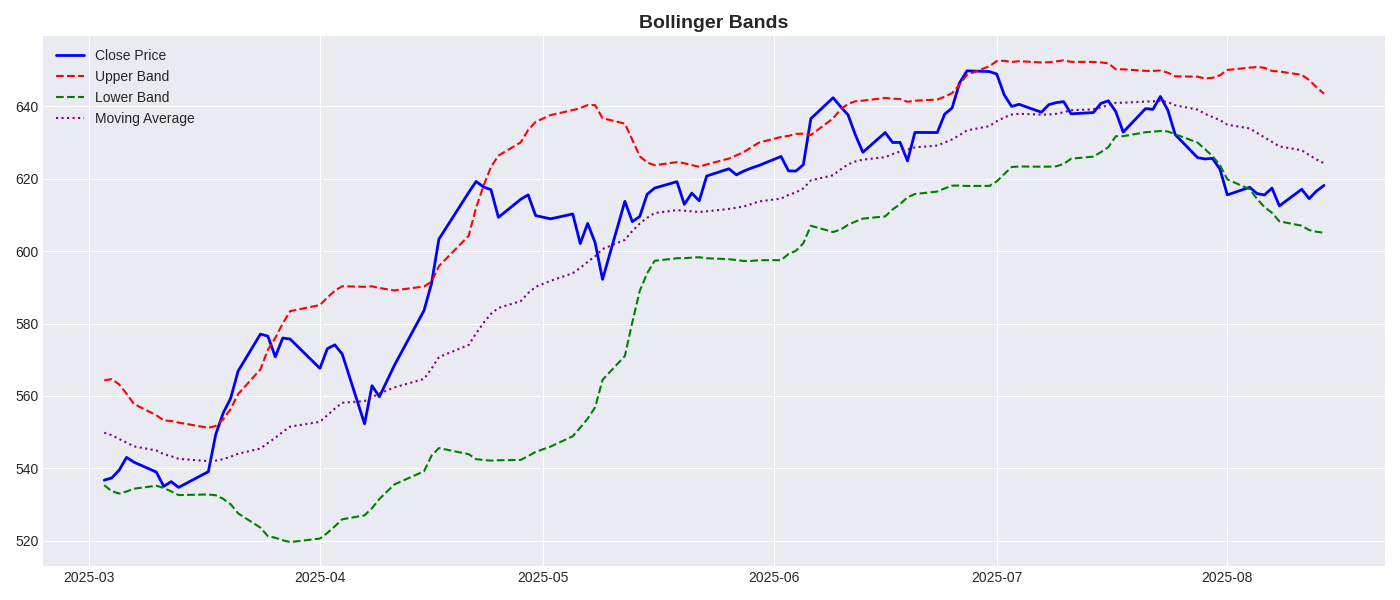
\includegraphics[width=0.8\textwidth]{../figures/input/bollinger.png}
    \caption{Illustrative example of Bollinger Bands showing upper, middle, and lower bands around price series.}
\end{figure}

The statistical rationale for Bollinger Bands is rooted in the assumption that returns approximate a normal distribution. Under this assumption, setting $k = 2$ should encompass approximately 95.45\% of observed prices within the bands. Thus, prices breaching the bands are statistically unusual events that may indicate overbought or oversold conditions. However, empirical evidence shows that financial return distributions are often leptokurtic and skewed, implying that extreme deviations occur more frequently than the normal model predicts.

Bollinger Bands are inherently adaptive due to their dependence on the rolling standard deviation. In periods of high volatility, $\sigma_t$ increases, widening the bands and accommodating larger price fluctuations. In low-volatility periods, $\sigma_t$ decreases, narrowing the bands and signalling potential upcoming volatility expansions, a phenomenon often referred to as the ``Bollinger Squeeze''. This adaptiveness makes them particularly suitable for comparing markets with different volatility profiles, such as emerging markets like India and more mature markets like the UK and US.

From an interpretive perspective, Bollinger Bands can be applied using two broad hypotheses. The first is the mean reversion hypothesis, where the Middle Band is treated as a dynamic equilibrium price. Prices near or outside the Upper Band may be deemed overbought and likely to revert downward, while prices near or below the Lower Band may be deemed oversold and likely to revert upward. The second is the trend continuation hypothesis, where band breaches in the direction of the prevailing trend are interpreted as signals of sustained momentum rather than imminent reversal. This dual interpretability means Bollinger Bands are non-directional and require contextual analysis or confirmation from other indicators.

In addition to the primary band structure, two derived measures are often employed to enhance interpretation. The first is the Bandwidth ($BW_t$), which measures the relative width of the bands:
\[
BW_t = \frac{UB_t - LB_t}{MB_t}
\]
Bandwidth serves as a normalized volatility measure, allowing for cross-asset and cross-market comparison of volatility conditions. Narrow bandwidth values are often precursors to volatility expansions, whereas wide bandwidths tend to occur during or just after high-volatility events.

The second is the \%B indicator, which quantifies the position of the current price within the bands:
\[
\%B_t = \frac{P_t - LB_t}{UB_t - LB_t}
\]
A value of $\%B_t = 1$ indicates that the price is at the Upper Band, $\%B_t = 0$ places it at the Lower Band, and values outside the range $[0, 1]$ indicate breaches beyond the respective band. This measure standardizes the interpretation of price location within the envelope and facilitates statistical analysis of band-related signals.

A numerical example illustrates the calculation process. Consider $n=5$, $k=2$, and the last five closing prices: $[100, 102, 101, 104, 103]$. The Middle Band is:
\[
MB_t = \frac{100 + 102 + 101 + 104 + 103}{5} = 102
\]
The deviations from the mean are $[-2, 0, -1, 2, 1]$, with squared deviations $[4, 0, 1, 4, 1]$. The variance is:
\[
\frac{4+0+1+4+1}{5} = 2
\]
Thus, the standard deviation is:
\[
\sigma_t = \sqrt{2} \approx 1.4142
\]
The Upper and Lower Bands become:
\[
UB_t = 102 + 2 \times 1.4142 \approx 104.8284
\]
\[
LB_t = 102 - 2 \times 1.4142 \approx 99.1716
\]
Any closing price above $\approx 104.83$ breaches the upper band, while any price below $\approx 99.17$ breaches the lower band.

The effectiveness of Bollinger Bands is highly sensitive to the chosen parameters $(n, k)$. Shorter $n$ values result in faster adaptation to price changes but increase susceptibility to noise, while longer $n$ values produce smoother bands at the cost of slower responsiveness. Similarly, smaller $k$ values tighten the bands, increasing the frequency of breaches, whereas larger $k$ values reduce breach frequency but risk missing early signals in emerging trends.

The strengths of Bollinger Bands include their adaptability to different volatility environments, ease of interpretation, and applicability to various asset classes and markets. They also provide a statistically grounded framework based on standard deviation, facilitating hypothesis testing in academic research. However, limitations include their lagging nature, inherent in moving averages, the assumption of normally distributed returns, and their sensitivity to parameter selection.






\subsubsection{Relative Strength Index (RSI)}
The Relative Strength Index (RSI), developed by J. Welles Wilder in 1978, is a momentum oscillator that measures the speed and magnitude of recent price changes to evaluate overbought or oversold conditions in the market. Unlike many price-based indicators, RSI is bounded between 0 and 100, making it easy to interpret and compare across assets and markets. The RSI is designed to quantify the relative strength of upward price movements against downward price movements over a specified look-back period, most commonly 14 periods. In the context of this dissertation, RSI serves as an essential measure of momentum across Indian, UK, and US publicly traded funds, offering a consistent and statistically definable signal for comparative performance analysis.

The RSI calculation begins with defining two core components: the average gain and the average loss over the look-back period. Let $P_t$ denote the closing price at time $t$, and $\Delta_t = P_t - P_{t-1}$ represent the price change from the previous period. The gain $G_t$ and loss $L_t$ for period $t$ are defined as:
\[
G_t = \max(\Delta_t, 0)
\]
\[
L_t = \max(-\Delta_t, 0)
\]
This separation ensures that gains are recorded as positive values when prices increase, and losses are recorded as positive values when prices decrease.

The next step involves calculating the average gain ($AG_t$) and average loss ($AL_t$) over the look-back period $n$. In Wilder's original method, a smoothed moving average—rather than a simple arithmetic mean—is used to maintain continuity in the calculation and to avoid abrupt changes when new data points are added. The initial averages are computed for the first $n$ periods as:
\[
AG_n = \frac{\sum_{i=1}^{n} G_i}{n}
\]
\[
AL_n = \frac{\sum_{i=1}^{n} L_i}{n}
\]
For subsequent periods $(t > n)$, Wilder's smoothing technique updates the averages as:
\[
AG_t = \frac{(AG_{t-1} \cdot (n-1)) + G_t}{n}
\]
\[
AL_t = \frac{(AL_{t-1} \cdot (n-1)) + L_t}{n}
\]
This smoothing formula behaves similarly to an exponential moving average, reducing the lag and providing a stable yet responsive measure of gains and losses.

Once the smoothed average gains and losses are computed, the Relative Strength (RS) is defined as:
\[
RS_t = \frac{AG_t}{AL_t}
\]
The RS value expresses how many times larger the average gain is compared to the average loss over the look-back period. When average losses approach zero, RS becomes large, driving RSI toward its upper bound of 100. Conversely, when average gains approach zero, RS becomes small, pushing RSI toward 0.

The RSI is then calculated using the transformation:
\[
RSI_t = 100 - \frac{100}{1 + RS_t}
\]
This formula ensures that $RSI_t$ is always bounded between 0 and 100. By construction, when gains equal losses ($RS_t = 1$), $RSI_t$ equals 50, representing a neutral momentum state. RSI values above 50 indicate average gains exceed average losses, while values below 50 indicate the opposite.


\begin{figure}[H]
    \centering
    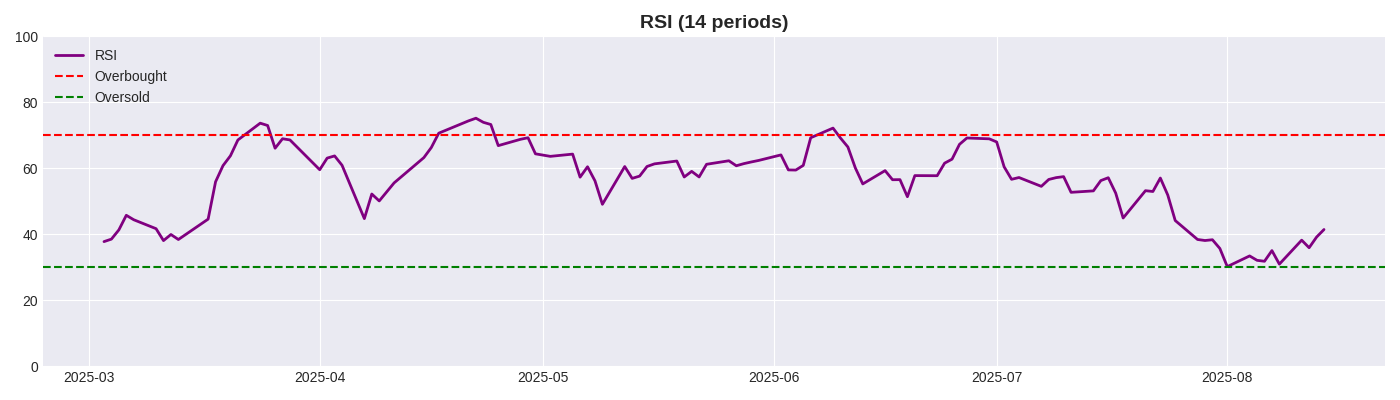
\includegraphics[width=0.7\textwidth]{../figures/input/rsi.png}
    \caption{Illustrative example of the Relative Strength Index (RSI) bounded between 0 and 100.}
\end{figure}


The bounded nature of RSI facilitates consistent interpretation:
\begin{itemize}
    \item RSI above 70 is typically interpreted as indicating overbought conditions, suggesting a possible reversal or price correction.
    \item RSI below 30 is typically interpreted as indicating oversold conditions, suggesting a potential rebound.
\end{itemize}
These threshold levels can be adjusted depending on asset volatility or market conditions—for example, using 80/20 thresholds for highly volatile assets to reduce false signals.

The statistical rationale behind RSI stems from its normalization of gains and losses over the look-back period. This normalization makes RSI scale-independent, allowing for direct comparison across instruments with different price ranges. The ratio form $(AG_t / AL_t)$ ensures that RSI reflects the balance between upward and downward momentum rather than absolute price levels.

Consider a worked example using $n=14$ periods. Suppose over the first 14 days, the sum of gains is 28 units, and the sum of losses is 14 units. The initial average gain is:
\[
AG_{14} = \frac{28}{14} = 2
\]
The initial average loss is:
\[
AL_{14} = \frac{14}{14} = 1
\]
Thus, the relative strength is:
\[
RS_{14} = \frac{2}{1} = 2
\]
The RSI is then:
\[
RSI_{14} = 100 - \frac{100}{1 + 2} = 100 - \frac{100}{3} \approx 66.67
\]
This value suggests bullish momentum but not yet overbought conditions. If, in subsequent periods, gains consistently outweigh losses, the smoothed averages will adjust, RS will increase, and RSI will move closer to 100.

From a time-series analysis perspective, RSI behaves as a momentum oscillator that filters out noise by smoothing gains and losses. It inherently captures mean-reverting tendencies: extreme high RSI values indicate strong recent upward moves that may be unsustainable, while extreme low values indicate strong downward moves that may similarly reverse. This property makes RSI particularly relevant for markets that oscillate between overbought and oversold states.

One of the mathematical strengths of RSI is that it adapts to different market volatilities without the need for explicit volatility measures. This is because gains and losses are computed in relative magnitude terms and smoothed over time, inherently adjusting to varying price dynamics. However, in highly volatile environments, RSI can remain in overbought or oversold territory for extended periods, which requires contextual interpretation and often the combination with trend-following indicators to avoid premature counter-trend trades.

The performance of RSI-based strategies can be affected by the choice of look-back period $n$. Shorter periods (e.g., $n=7$) make RSI more sensitive to recent price changes, generating more frequent signals but increasing noise and false positives. Longer periods (e.g., $n=21$ or $n=30$) produce smoother RSI values, reducing noise but potentially delaying signals. In academic testing, the standard $n=14$ has provided a balance between sensitivity and stability, but optimization for specific markets can yield better results.

RSI can also be modified through signal line crossovers, divergence analysis, and dynamic thresholding. Divergence occurs when price makes a new high or low not confirmed by RSI, often interpreted as a weakening trend and a potential reversal point. Mathematically, divergence detection involves correlating the slope of the price series with the slope of the RSI series over the same interval and identifying mismatches in directional movement.

In a cross-market study such as this dissertation, RSI offers several advantages:
\begin{enumerate}
    \item Its bounded scale allows for direct cross-country comparisons regardless of price level differences between Indian, UK, and US funds.
    \item The normalization process implicitly adjusts for differences in volatility across markets.
    \item It is computationally straightforward, reducing the potential for implementation errors in large-scale backtesting.
\end{enumerate}





\subsubsection{Moving Average Convergence Divergence (MACD)}

The Moving Average Convergence Divergence (MACD) indicator, developed by Gerald Appel in the late 1970s, is a trend-following momentum oscillator that measures the relationship between two exponentially smoothed moving averages of an asset’s price. Its primary objective is to reveal changes in the strength, direction, momentum, and duration of a trend. Unlike simple moving averages (SMA), which apply equal weighting to all observations in the look-back period, the MACD relies on Exponential Moving Averages (EMA), which assign greater weight to more recent prices, thereby responding more quickly to new market information. This responsiveness makes the MACD suitable for detecting both short-term and long-term trend shifts, and its structure also allows it to serve as a momentum gauge through the use of a signal line and histogram.

Mathematically, the MACD line at time $t$ is computed as the difference between two EMAs of the price series $P_t$:
\[
MACD_t = EMA_{t}^{(s)} - EMA_{t}^{(l)}
\]
where:
\begin{itemize}
    \item $EMA_{t}^{(s)}$ is the short-term EMA of length $s$ periods (typically $s=12$ for daily data),
    \item $EMA_{t}^{(l)}$ is the long-term EMA of length $l$ periods (typically $l=26$).
\end{itemize}
The EMA is defined recursively as:
\[
EMA_t^{(n)} = \alpha_n P_t + (1 - \alpha_n) EMA_{t-1}^{(n)}
\]
with the smoothing constant:
\[
\alpha_n = \frac{2}{n+1}
\]
The initial EMA value can be seeded by the SMA of the first $n$ observations:
\[
EMA_{n}^{(n)} = \frac{1}{n} \sum_{i=0}^{n-1} P_{n-i}
\]
In this formulation, more recent prices have exponentially greater influence, with the weighting factor $(1-\alpha_n)^k$ assigned to the price $k$ periods in the past.

Once the MACD line is computed, a signal line is generated as the EMA of the MACD values themselves over a shorter smoothing period $p$ (typically $p=9$):
\[
Signal_t = EMA_{t}^{(p)}(MACD)
\]
The signal line serves as a trigger for buy and sell signals based on crossovers with the MACD line:
\begin{itemize}
    \item Bullish signal: $MACD_t$ crosses above $Signal_t$.
    \item Bearish signal: $MACD_t$ crosses below $Signal_t$.
\end{itemize}

The third component of the MACD framework is the histogram, which represents the difference between the MACD line and the signal line:
\[
Histogram_t = MACD_t - Signal_t
\]
The histogram visually quantifies the convergence or divergence between the MACD and its signal line:
\begin{itemize}
    \item Positive histogram values indicate that the MACD is above the signal line, suggesting bullish momentum.
    \item Negative histogram values indicate that the MACD is below the signal line, suggesting bearish momentum.
\end{itemize}
The magnitude of the histogram reflects the strength of the divergence, serving as a momentum amplifier.

\begin{figure}[H]
    \centering
    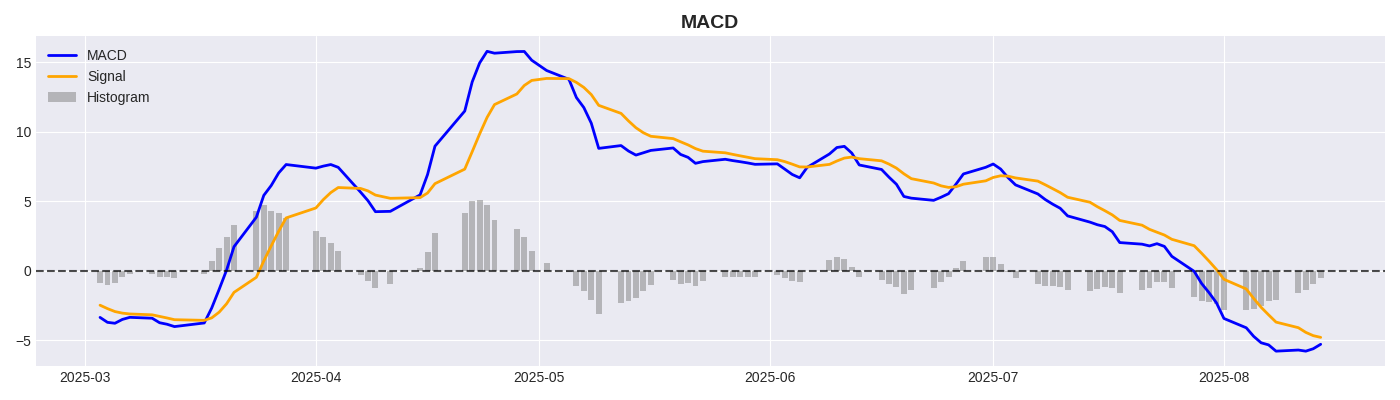
\includegraphics[width=0.7\textwidth]{../figures/input/macd.png}
    \caption{Illustrative example of the Relative Strength Index (RSI) bounded between 0 and 100.}
\end{figure}

The interpretive foundation of the MACD lies in the notions of convergence and divergence:
\begin{itemize}
    \item Convergence occurs when the short-term and long-term EMAs move toward each other, implying weakening momentum.
    \item Divergence occurs when they move apart, implying strengthening momentum.
\end{itemize}
Because EMAs themselves are smoothed averages, the MACD line represents a smoothed differential measure of price momentum, reducing noise compared to raw price changes.

From a statistical perspective, the EMA is a form of low-pass filter in time-series analysis, attenuating high-frequency fluctuations while preserving low-frequency trend components. By taking the difference of two EMAs with distinct lengths, the MACD acts as a band-pass filter, isolating intermediate-term cycles in price data. The signal line, being another EMA applied to the MACD series, further smooths the output, making it easier to identify meaningful shifts in trend momentum.

To illustrate the calculation, consider daily closing prices $\{P_t\}$ over 30 days, with parameters $s=12$, $l=26$, and $p=9$. The steps are:
\begin{enumerate}
    \item Calculate the 12-day EMA of $P_t$:
    \[
    EMA_t^{(12)} = \frac{2}{13} P_t + \frac{11}{13} EMA_{t-1}^{(12)}
    \]
    \item Calculate the 26-day EMA of $P_t$:
    \[
    EMA_t^{(26)} = \frac{2}{27} P_t + \frac{25}{27} EMA_{t-1}^{(26)}
    \]
    \item Subtract the 26-day EMA from the 12-day EMA to obtain the MACD line:
    \[
    MACD_t = EMA_t^{(12)} - EMA_t^{(26)}
    \]
    \item Calculate the 9-day EMA of the MACD series to obtain the signal line:
    \[
    Signal_t = \frac{2}{10} MACD_t + \frac{8}{10} Signal_{t-1}
    \]
    \item Compute the histogram:
    \[
    Histogram_t = MACD_t - Signal_t
    \]
\end{enumerate}
In practical use, these values are recalculated sequentially for each time step, with initial EMA values derived from the SMA of the first $n$ prices.

The MACD's strength lies in its ability to combine trend-following and momentum properties. The difference between the short-term and long-term EMAs captures the direction and strength of the trend, while the signal line crossovers provide actionable trading triggers. Additionally, the histogram offers a clear visual cue of changes in momentum, often preceding actual crossovers.

Despite its popularity, the MACD has limitations. As a lagging indicator, it relies on historical price data, meaning that signals are generated after a trend has begun and may be late during rapid reversals. Whipsaws—false signals during ranging markets—are common. Parameter sensitivity is another issue: shorter EMA lengths increase responsiveness but also noise, while longer lengths smooth fluctuations but delay signals. There is no universally optimal set of parameters; empirical testing across markets and timeframes is necessary to adapt the MACD to specific contexts.

From a probabilistic standpoint, the MACD's crossover signals implicitly assume that momentum changes have persistence—i.e., that recent acceleration in price will continue over subsequent periods. This assumption may hold in trending markets but fails in highly mean-reverting environments. Thus, statistical validation of MACD-based signals requires performance analysis under distinct volatility and trend regimes.

In the cross-market context of Indian, UK, and US funds, the MACD offers a standardized momentum measure that can be applied with consistent parameters across diverse volatility environments. Because emerging markets like India often exhibit higher volatility, the magnitude and frequency of histogram extremes may differ significantly from those in mature markets such as the UK and US. This characteristic makes the MACD a valuable tool for comparative performance analysis, provided its outputs are normalized for volatility differences.

Mathematically, the MACD can also be interpreted as an approximation of the derivative of a smoothed price series. Let $S_t^{(l)}$ denote the long EMA; the short EMA $S_t^{(s)}$ responds faster to price changes, so $MACD_t = S_t^{(s)} - S_t^{(l)}$ approximates the slope of the long-term trend. The signal line, being a smoothed version of this slope, serves as a noise filter, while the histogram represents the difference between the raw slope estimate and its smoothed version, thereby isolating short-term momentum deviations from the longer-term baseline.

To further quantify the responsiveness of the MACD, consider its impulse response function derived from the EMA's weighting scheme. For the short EMA:
\[
w_k^{(s)} = \alpha_s (1 - \alpha_s)^k, \quad k \ge 0
\]
and for the long EMA:
\[
w_k^{(l)} = \alpha_l (1 - \alpha_l)^k
\]
The MACD weights are:
\[
w_k^{(MACD)} = w_k^{(s)} - w_k^{(l)}
\]
These weights sum to zero, indicating that the MACD acts as a high-pass filter relative to the long EMA and a low-pass filter relative to the short EMA. The signal line applies a second exponential smoothing to $w_k^{(MACD)}$, further attenuating high-frequency noise.

In practice, MACD analysis often incorporates divergences between the MACD line and price action:
\begin{itemize}
    \item Bullish divergence: Price makes a lower low, but MACD forms a higher low.
    \item Bearish divergence: Price makes a higher high, but MACD forms a lower high.
\end{itemize}
Such divergences suggest weakening momentum and potential trend reversals, though they are probabilistic rather than deterministic signals.


\subsubsection{Ichimoku Clouds}

Ichimoku Clouds, also known as Ichimoku Kinko Hyo, is a comprehensive technical indicator developed by Goichi Hosoda in the late 1930s and published in 1969. The term “Ichimoku Kinko Hyo” translates to “one glance equilibrium chart,” reflecting the indicator’s ability to provide an immediate view of market trend, momentum, and potential support and resistance levels. Unlike single-line indicators, Ichimoku Clouds incorporate multiple components that together form a dynamic picture of price action, combining moving averages of varying lengths with forward and backward projections.

Mathematically, the Ichimoku system consists of five primary lines: the Tenkan-sen (Conversion Line), the Kijun-sen (Base Line), the Senkou Span A (Leading Span A), the Senkou Span B (Leading Span B), and the Chikou Span (Lagging Span). The shaded region between Senkou Span A and Senkou Span B is referred to as the “cloud” or “Kumo,” which serves as a key visual element indicating potential areas of support and resistance.

Let $H_t$, $L_t$, and $C_t$ denote the high, low, and closing prices at time $t$, respectively. The Ichimoku components are defined as follows:

1. Tenkan-sen (Conversion Line):
\[
\text{Tenkan-sen}_t = \frac{\max(H_{t-(p_1-1)}, \dots, H_t) + \min(L_{t-(p_1-1)}, \dots, L_t)}{2}
\]
where $p_1$ is the look-back period for the Tenkan-sen, typically $p_1 = 9$ periods in the default configuration. This represents the midpoint between the highest high and lowest low over the past $p_1$ periods, serving as a short-term trend indicator.

2. Kijun-sen (Base Line):
\[
\text{Kijun-sen}_t = \frac{\max(H_{t-(p_2-1)}, \dots, H_t) + \min(L_{t-(p_2-1)}, \dots, L_t)}{2}
\]
where $p_2$ is the look-back period for the Kijun-sen, typically $p_2 = 26$ periods. This represents the midpoint between the highest high and lowest low over a longer period than the Tenkan-sen, serving as an intermediate trend indicator and a benchmark for momentum shifts.

3. Senkou Span A (Leading Span A):
\[
\text{Senkou Span A}_t = \frac{\text{Tenkan-sen}_t + \text{Kijun-sen}_t}{2}
\]
This is plotted forward by $p_2$ periods from the current time, providing a forward-looking boundary of the cloud. It is a dynamic average of short- and medium-term trends, projected into the future.

4. Senkou Span B (Leading Span B):
\[
\text{Senkou Span B}_t = \frac{\max(H_{t-(p_3-1)}, \dots, H_t) + \min(L_{t-(p_3-1)}, \dots, L_t)}{2}
\]
where $p_3$ is the look-back period for the Senkou Span B calculation, typically $p_3 = 52$ periods. This is also plotted forward by $p_2$ periods. Senkou Span B tends to move more slowly than Senkou Span A and provides a longer-term view of equilibrium price levels.

5. Chikou Span (Lagging Span):
\[
\text{Chikou Span}_t = C_{t}
\]
plotted backward by $p_2$ periods. This represents the current closing price displaced into the past, allowing for quick visual comparison of current price relative to historical price action.

The cloud (Kumo) itself is the area between Senkou Span A and Senkou Span B:
\[
\text{Kumo}_t = \{\text{area between Senkou Span A}_t \ \text{and} \ \text{Senkou Span B}_t\}
\]
When Senkou Span A is above Senkou Span B, the cloud is typically shaded one color (often green), indicating bullish conditions. When Senkou Span A is below Senkou Span B, the cloud is shaded another color (often red), indicating bearish conditions.

The default parameter values $(p_1, p_2, p_3) = (9, 26, 52)$ originate from Japanese trading practices of the time, where a 9-period span approximated 1.5 weeks of trading days, 26 periods approximated one month, and 52 approximated two months in a six-day trading week environment. These parameters have been retained in modern five-day trading weeks due to their proven balance between responsiveness and stability.

\begin{figure}[H]
    \centering
    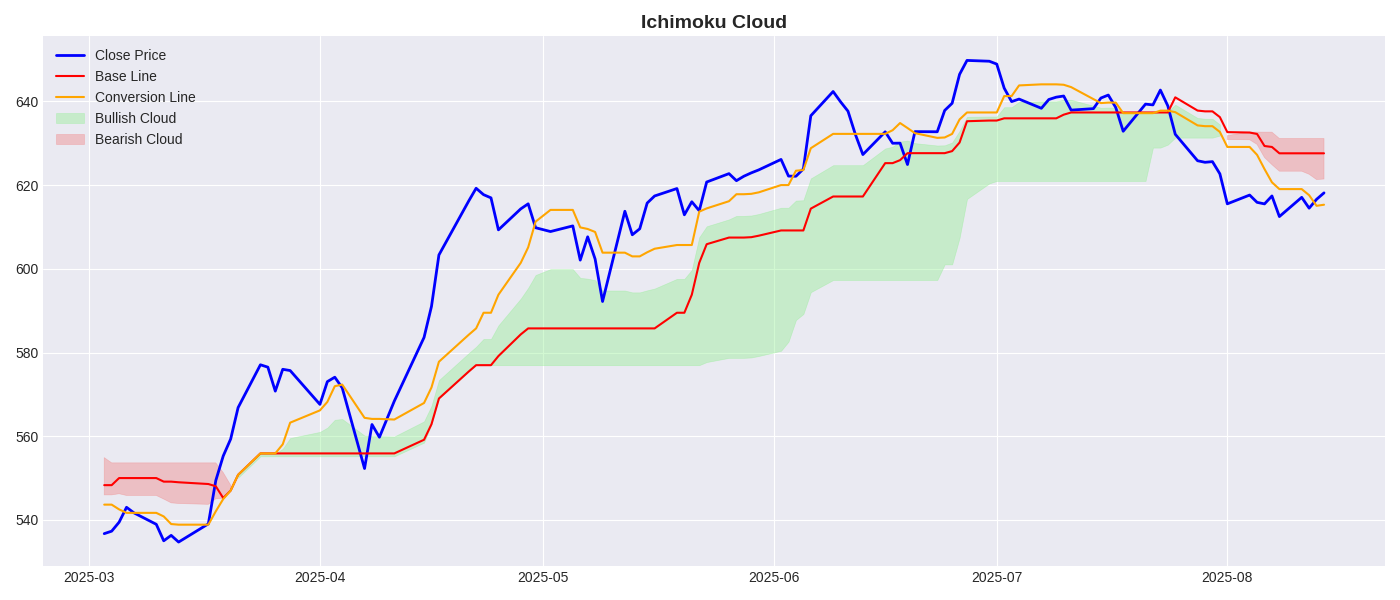
\includegraphics[width=0.7\textwidth]{../figures/input/ichimoku.png}
    \caption{Illustrative example of the Relative Strength Index (RSI) bounded between 0 and 100.}
\end{figure}

From a statistical standpoint, the Tenkan-sen and Kijun-sen are not traditional moving averages but midpoints of high-low ranges, making them more robust to extreme price outliers compared to simple or exponential moving averages. By focusing on midpoints, Ichimoku lines can provide a smoother representation of equilibrium levels while preserving sensitivity to directional changes in price extremes.

Interpretation of Ichimoku Clouds relies on the interaction of these components. Price above the Kumo generally signals bullish conditions; price below the Kumo signals bearish conditions. Crossovers between the Tenkan-sen and Kijun-sen can indicate momentum shifts, with bullish crossovers occurring when the Tenkan-sen crosses above the Kijun-sen, and bearish crossovers when the opposite occurs. The thickness of the Kumo reflects volatility and the strength of support or resistance; a thicker Kumo is harder for price to break through, while a thinner Kumo is more easily penetrated. The Chikou Span’s position relative to historical price offers confirmation: if it is above historical prices, bullish sentiment is reinforced; if below, bearish sentiment is reinforced. The forward projection of Senkou Span A and B allows traders to anticipate future support or resistance zones, unlike most lagging indicators.

Mathematically, one can quantify the Kumo thickness as:
\[
\text{Kumo Width}_t = |\text{Senkou Span A}_t - \text{Senkou Span B}_t|
\]
This can be normalized by dividing by current price or an average price level to facilitate comparison across assets with different price scales:
\[
\text{Normalized Kumo Width}_t = \frac{|\text{Senkou Span A}_t - \text{Senkou Span B}_t|}{C_t}
\]
A higher normalized width implies stronger projected support or resistance, while a lower width implies weaker zones.

In empirical testing, signal generation can be expressed algorithmically using logical conditions. For example, a bullish signal might be defined as:
\[
\text{Buy Signal at time } t \iff ( \text{Tenkan-sen}_t > \text{Kijun-sen}_t ) \land 
\]
\[
( C_t > \max(\text{Senkou Span A}_t, \text{Senkou Span B}_t) ) \land ( \text{Chikou Span}_t > \text{Price}_{t-p_2} )
\]
Conversely, a bearish signal might require:
\[
\text{Sell Signal at time } t \iff ( \text{Tenkan-sen}_t < \text{Kijun-sen}_t ) \land 
\]
\[
( C_t < \min(\text{Senkou Span A}_t, \text{Senkou Span B}_t) ) \land ( \text{Chikou Span}_t < \text{Price}_{t-p_2} )
\]
These conditions combine trend direction, price location relative to the cloud, and historical confirmation.

From a volatility-adjusted perspective, the forward-projected Kumo can be interpreted as a confidence interval for future price equilibrium. While not statistically derived like Bollinger Bands, the concept is similar: the cloud's width expands in volatile periods (greater high-low range in the past) and contracts in stable periods.

The multi-timeframe nature of Ichimoku Clouds arises from the interaction of $p_1$, $p_2$, and $p_3$. Tenkan-sen reacts to short-term price extremes, Kijun-sen reflects intermediate-term structure, and Senkou Span B incorporates a longer-term equilibrium. By combining these elements, the indicator effectively embeds three overlapping horizons into a single visual framework.

In cross-market research such as the comparison of Indian, UK, and US publicly traded funds, Ichimoku Clouds offer distinctive advantages. Their reliance on price extremes rather than averages allows them to adapt to markets with different volatility profiles. The forward-projected cloud provides a comparative measure of anticipated support or resistance that can be statistically analyzed across markets. Kumo thickness and cloud color transitions can be used to quantify regime changes, allowing objective classification of bullish, bearish, and neutral phases.

One can define regime states mathematically by assigning:
\[
\text{Regime}_t =
\begin{cases}
1 & \text{if } C_t > \max(\text{Senkou Span A}_t, \text{Senkou Span B}_t) \\
-1 & \text{if } C_t < \min(\text{Senkou Span A}_t, \text{Senkou Span B}_t) \\
0 & \text{otherwise}
\end{cases}
\]
This representation enables statistical testing of return distributions conditional on regime state, facilitating hypothesis testing about the predictive value of Ichimoku-derived signals.

\subsection{Signal Generation and Trading Strategy}

Signal generation forms the critical link between indicator calculation and the implementation of a systematic trading strategy. While technical indicators such as Bollinger Bands, RSI, MACD, and Ichimoku Clouds quantify different aspects of price dynamics—volatility, momentum, and trend—signals translate these continuous mathematical measures into discrete trading decisions. The process involves defining logical conditions based on indicator values and price action, which trigger actionable states such as ``Buy'', ``Sell'', or ``Hold''. This transformation from continuous variables to discrete states is essential for backtesting, portfolio construction, and real-world execution.

Mathematically, a trading signal can be defined as a function:
\[
S_t = f(\mathcal{I}_t, \Theta)
\]
where $\mathcal{I}_t$ is the vector of indicator values at time $t$ and $\Theta$ represents the parameter set governing thresholds, look-back periods, and other tunable variables. The output $S_t \in \{-1, 0, 1\}$ typically denotes:
\begin{itemize}
    \item $S_t = 1$: Buy or go long.
    \item $S_t = -1$: Sell or go short.
    \item $S_t = 0$: Hold or no position change.
\end{itemize}
In a long-only fund strategy, $S_t = -1$ may correspond to closing an existing position or shifting to cash.

\subsubsection{Threshold-Based Signals}

Threshold-based rules directly map indicator values to trading actions. For example, an RSI strategy with thresholds $\tau_{\text{low}}$ and $\tau_{\text{high}}$ can be written as:
\[
S_t =
\begin{cases}
1 & \text{if } RSI_t < \tau_{\text{low}} \\
-1 & \text{if } RSI_t > \tau_{\text{high}} \\
0 & \text{otherwise}
\end{cases}
\]
This approach exploits overbought/oversold interpretations. The symmetry of the decision boundaries facilitates statistical testing: one can compute conditional returns given $RSI_t$ in specific zones to evaluate predictive value.

\subsubsection{Crossover Signals}

Crossover rules compare two time series, often a faster and a slower measure, to identify shifts in momentum or trend. Mathematically, a simple moving average (SMA) crossover signal is:
\[
S_t =
\begin{cases}
1 & \text{if } MA^{(f)}_t > MA^{(s)}_t \ \text{and} \ MA^{(f)}_{t-1} \le MA^{(s)}_{t-1} \\
-1 & \text{if } MA^{(f)}_t < MA^{(s)}_t \ \text{and} \ MA^{(f)}_{t-1} \ge MA^{(s)}_{t-1} \\
0 & \text{otherwise}
\end{cases}
\]
where $MA^{(f)}$ and $MA^{(s)}$ denote the fast and slow moving averages. This structure generalises to MACD–signal line crossovers and Tenkan-sen–Kijun-sen crossovers in Ichimoku analysis.

\subsubsection{Price–Indicator Relationship Rules}

Some strategies trigger signals when price interacts with an indicator-derived level, such as Bollinger Bands. A mean reversion variant is:
\[
S_t =
\begin{cases}
1 & \text{if } P_t < LB_t \\
-1 & \text{if } P_t > UB_t \\
0 & \text{otherwise}
\end{cases}
\]
A trend-following variant inverts this logic: buying on upper band breaches and selling on lower band breaches. Mathematically, both can be unified by defining a polarity parameter $\phi \in \{-1, 1\}$:
\[
S_t = \phi \cdot \mathbf{1}_{(P_t > UB_t)} - \phi \cdot \mathbf{1}_{(P_t < LB_t)}
\]
where $\mathbf{1}_{(\cdot)}$ is the indicator function.

\subsubsection{Multi-Condition Rules}

More robust signals often combine multiple indicator conditions to filter noise. For example, a bullish Ichimoku signal can be formalised as:
\[
S_t =
\begin{cases}
1 & \text{if } (\text{Tenkan}_t > \text{Kijun}_t) \land (P_t > \max(SA_t, SB_t)) \land (\text{Chikou}_t > P_{t-p_2}) \\
-1 & \text{if } (\text{Tenkan}_t < \text{Kijun}_t) \land (P_t < \min(SA_t, SB_t)) \land (\text{Chikou}_t < P_{t-p_2}) \\
0 & \text{otherwise}
\end{cases}
\]
where $SA_t$ and $SB_t$ are Senkou Span A and B.

\subsubsection{Signal Smoothing}

Raw signal generation can produce whipsaws in choppy markets. One method to mitigate this is applying a persistence filter: require that a signal condition be met for $m$ consecutive periods before acting. Let $C_t$ be the binary condition for a buy signal at time $t$; then the smoothed signal is:
\[
S_t =
\begin{cases}
1 & \text{if } \sum_{i=0}^{m-1} C_{t-i} = m \\
0 & \text{otherwise}
\end{cases}
\]
This filter can be applied symmetrically for sell conditions.

\subsubsection{Position Management and Trade Execution}

Once a signal is generated, the trading strategy must define:
\begin{itemize}
    \item \textit{Entry Rules}: At what price and volume to enter upon a buy or sell signal. Often modelled as entering at next period's open price.
    \item \textit{Exit Rules}: Opposite signal triggers, fixed holding periods, or stop-loss/take-profit thresholds.
    \item \textit{Position Sizing}: Fraction of capital to commit, denoted $\omega_t$, which may be fixed (e.g., $\omega_t = 1$ for full allocation) or variable based on conviction, volatility, or risk parity.
\end{itemize}
If transaction costs are $c$ per trade, the realised return from a signal-based trade opened at $P_e$ and closed at $P_x$ is:
\[
R_{\text{net}} = \frac{P_x - P_e}{P_e} \cdot \text{dir} - 2c
\]
where $\text{dir} \in \{1, -1\}$ is the trade direction.

\subsubsection{Backtesting Framework}

In a discrete-time backtest with $T$ periods, the strategy return series $\{r_t^{(S)}\}$ is computed as:
\[
r_t^{(S)} = S_{t-1} \cdot \frac{P_t - P_{t-1}}{P_{t-1}} - \gamma \cdot |S_t - S_{t-1}|
\]
where $\gamma$ is the per-unit transaction cost and $|S_t - S_{t-1}|$ captures position changes (0 for hold, 1 for entry/exit, 2 for reversal).

Cumulative return is then:
\[
CR_T = \prod_{t=1}^T (1 + r_t^{(S)}) - 1
\]
Risk-adjusted performance is assessed via the Sharpe Ratio:
\[
\text{Sharpe} = \frac{\overline{r^{(S)}} - r_f}{\sigma_{r^{(S)}}}
\]
where $r_f$ is the risk-free rate (often set to 0 in short-term tests).

\subsubsection{Regime-Based Signal Evaluation}

To account for market heterogeneity across Indian, UK, and US funds, signal efficacy can be tested conditionally on volatility or trend regimes. Let $V_t$ be a volatility state variable (e.g., high/low from a Markov-switching model) and $R_t$ be the regime label. The conditional mean return for buy signals is:
\[
\mu_{\text{buy}, r} = \frac{\sum_{t=1}^T \mathbf{1}_{(S_t=1, R_t=r)} \cdot r_t}{\sum_{t=1}^T \mathbf{1}_{(S_t=1, R_t=r)}}
\]
where $r$ indexes regimes. This decomposition quantifies whether signals are more effective in trending versus ranging or high- versus low-volatility states.

\subsubsection{Statistical Significance Testing}

The profitability of a trading signal can be evaluated using a one-sample $t$-test on its conditional returns:
\[
t_{\text{stat}} = \frac{\overline{r^{(S)}}}{\sigma_{r^{(S)}} / \sqrt{N}}
\]
where $N$ is the number of trades. A significant $t_{\text{stat}}$ (beyond chosen critical values) suggests that average trade returns differ from zero, adjusting for sample variability.

Alternatively, a binomial test can be applied to the proportion of winning trades $p_{\text{win}}$ under the null hypothesis $p_{\text{win}} = 0.5$:
\[
z = \frac{p_{\text{win}} - 0.5}{\sqrt{0.25 / N}}
\]

\subsubsection{Integration Across Indicators}

Finally, multi-indicator strategies aggregate signals to reduce false positives. Let $S_t^{(i)}$ denote the signal from indicator $i$. An ensemble signal could be:
\[
S_t^{(\text{agg})} = 
\begin{cases}
1 & \text{if } \sum_{i=1}^M S_t^{(i)} > \delta \\
-1 & \text{if } \sum_{i=1}^M S_t^{(i)} < -\delta \\
0 & \text{otherwise}
\end{cases}
\]
where $M$ is the number of indicators and $\delta$ is the decision threshold. For instance, $\delta = 2$ in a four-indicator system requires at least three agreeing signals to trade, enhancing reliability at the cost of fewer trades.


\subsection{Performance Measurement}

Performance measurement in the context of trading strategies refers to the systematic evaluation of returns, risk, and risk-adjusted returns generated by a given set of trading rules over a specified time period. The objective is to determine not only whether a strategy is profitable, but also whether its returns are statistically significant, robust, and justified relative to the risk undertaken. For this dissertation, where Bollinger Bands, RSI, MACD, and Ichimoku Clouds are applied to Indian, UK, and US publicly traded funds, performance measurement provides the empirical foundation for comparing the relative effectiveness of each indicator in different markets and volatility regimes.

At the core of performance evaluation lies the return series $\{r_t\}_{t=1}^T$ generated by the trading strategy. For a discrete-time backtest, assuming positions are entered and exited at observable market prices without slippage, the single-period simple return at time $t$ is:
\[
r_t = \frac{P_t - P_{t-1}}{P_{t-1}}
\]
where $P_t$ denotes the asset price (or portfolio value) at time $t$. In a signal-based strategy, returns are conditioned on position direction:
\[
r_t^{(S)} = S_{t-1} \cdot \frac{P_t - P_{t-1}}{P_{t-1}}
\]
where $S_{t-1} \in \{-1, 0, 1\}$ is the trading signal from the previous period. Transaction costs $c$ per trade can be incorporated as:
\[
r_t^{(S,net)} = S_{t-1} \cdot \frac{P_t - P_{t-1}}{P_{t-1}} - c \cdot |S_t - S_{t-1}|
\]
where $|S_t - S_{t-1}|$ counts the number of position changes (0 for hold, 1 for entry/exit, 2 for reversal).

\subsubsection{Cumulative Return}  
The total growth of capital over $T$ periods is expressed as the cumulative return:
\[
CR_T = \prod_{t=1}^T (1 + r_t^{(S,net)}) - 1
\]
Cumulative returns provide a straightforward measure of profitability but do not adjust for volatility or time horizon.

\subsubsection{Annualized Return}  
To standardize performance across assets with different backtest lengths, annualized returns are computed. If $N$ is the number of trading periods in a year (e.g., $N=252$ for daily data):
\[
AR = \left( \prod_{t=1}^T (1 + r_t^{(S,net)}) \right)^{\frac{N}{T}} - 1
\]
This facilitates comparisons across markets and strategies.

\subsubsection{Volatility}  
Risk is often proxied by the standard deviation of returns:
\[
\sigma_r = \sqrt{\frac{1}{T-1} \sum_{t=1}^T \left(r_t^{(S,net)} - \overline{r^{(S,net)}}\right)^2}
\]
Annualized volatility is:
\[
\sigma_{ann} = \sigma_r \cdot \sqrt{N}
\]
Volatility captures the dispersion of returns and is central to risk-adjusted metrics.

\subsubsection{Sharpe Ratio}  
The Sharpe Ratio (Sharpe, 1966) measures excess return per unit of risk:
\[
\text{Sharpe} = \frac{\overline{r^{(S,net)}} - r_f}{\sigma_r}
\]
where $r_f$ is the risk-free rate (often set to 0 for short-term tests). The annualized Sharpe Ratio is:
\[
\text{Sharpe}_{ann} = \frac{AR - r_f}{\sigma_{ann}}
\]
A higher Sharpe Ratio indicates better risk-adjusted performance. In cross-market analysis, it provides a scale-independent measure of relative efficiency.

\subsubsection{Sortino Ratio}  
While the Sharpe Ratio penalizes upside and downside volatility equally, the Sortino Ratio considers only downside deviation:
\[
\sigma_d = \sqrt{\frac{1}{T_d} \sum_{t: r_t^{(S,net)} < MAR} (r_t^{(S,net)} - MAR)^2}
\]
where $MAR$ is the minimum acceptable return and $T_d$ is the number of downside periods. The Sortino Ratio is:
\[
\text{Sortino} = \frac{\overline{r^{(S,net)}} - MAR}{\sigma_d}
\]
This is useful for strategies with asymmetric return distributions.

\subsubsection{Maximum Drawdown (MDD)}  
Drawdown quantifies the largest peak-to-trough decline in cumulative returns:
\[
DD_t = \frac{V_{\text{peak}} - V_t}{V_{\text{peak}}}
\]
where $V_t$ is the portfolio value at $t$ and $V_{\text{peak}}$ is the maximum historical value before $t$. The maximum drawdown is:
\[
MDD = \max_{t} DD_t
\]
MDD captures tail risk and strategy resilience during market stress.

\subsubsection{Calmar Ratio}  
The Calmar Ratio measures return relative to maximum drawdown:
\[
\text{Calmar} = \frac{AR}{|MDD|}
\]
A higher Calmar Ratio indicates more favorable return-to-drawdown characteristics.

\subsubsection{Win Rate and Profit Factor}  
Win rate is the proportion of profitable trades:
\[
\text{Win Rate} = \frac{\text{\# profitable trades}}{\text{\# total trades}}
\]
Profit factor is the ratio of gross profits to gross losses:
\[
\text{PF} = \frac{\sum_{\text{winning trades}} R_i}{\left| \sum_{\text{losing trades}} R_i \right|}
\]
These are intuitive metrics for evaluating signal accuracy.

\subsubsection{Risk-Adjusted Return Over Maximum Drawdown (RoMaD)}  
An alternative to the Sharpe Ratio, RoMaD is:
\[
\text{RoMaD} = \frac{AR}{|MDD|}
\]
Unlike Sharpe, RoMaD uses drawdown instead of volatility as the risk denominator.

\subsubsection{Alpha and Beta}  
If $r_m$ denotes market returns, alpha ($\alpha$) and beta ($\beta$) from the CAPM regression:
\[
r_t^{(S)} - r_f = \alpha + \beta (r_{m,t} - r_f) + \epsilon_t
\]
quantify the strategy's market-independent performance ($\alpha$) and market exposure ($\beta$).

\subsection{Our Trading Strategy Algorithm}

The trading strategy implemented in this study employs a systematic approach to signal generation and portfolio management across four distinct technical indicators. The algorithm operates on daily OHLCV data spanning five years for each fund, generating standardized buy and sell signals that are then evaluated for performance across Indian, UK, and US markets. The strategy follows a long-only approach, consistent with the nature of mutual funds and ETFs under examination.

\subsubsection{Algorithm Overview}

The core algorithm is designed as a modular pipeline that takes raw financial time series data, applies chosen technical indicators with predefined parameters, generates corresponding trading signals, and subsequently evaluates these signals through performance metrics. It can be mathematically represented as a multi-stage mapping:
\[
\mathcal{A}: (\mathbf{P}, \mathbf{I}, \Theta) \rightarrow (\mathbf{S}, \mathbf{R}, \mathbf{M})
\]
where:
\begin{itemize}
    \item $\mathbf{P} = \{O_t, H_t, L_t, C_t, V_t\}_{t=1}^T$ represents the OHLCV price matrix.
    \item $\mathbf{I} = \{BB, RSI, MACD, ICH\}$ denotes the set of technical indicators.
    \item $\Theta$ is the parameter space for each indicator (look-back periods, thresholds, smoothing constants).
    \item $\mathbf{S}$ is the generated signal matrix, with entries corresponding to buy, sell, or hold decisions.
    \item $\mathbf{R}$ is the realized return series based on executed trades.
    \item $\mathbf{M}$ contains aggregated performance metrics such as total return, Sharpe ratio, and win rate.
\end{itemize}

\subsubsection{Data Preprocessing and Validation}

Before any signal generation can occur, the raw OHLCV data must be prepared to ensure integrity and consistency across markets. This preprocessing stage removes non-trading days, fills missing values to maintain continuous time series, and validates the logical relationships between open, high, low, and close prices. Outliers in daily returns are flagged using a $3\sigma$ rule, reducing the risk of abnormal price spikes distorting indicator values. The resulting dataset is clean, aligned across all instruments, and suitable for subsequent technical analysis.

\begin{breakablealgorithm}
\caption{Data Preprocessing Module}
\begin{algorithmic}[1]
\Require Raw OHLCV data for each fund
\Ensure Clean, validated price series
\State {Load OHLCV data from Yahoo Finance API \Comment{Retrieve historical daily data}}
\State {Remove non-trading days and align time series \Comment{Ensure time consistency across markets}}
\State {Handle missing values using forward-fill methodology \Comment{Fill gaps with last available value}}
\State {Validate data integrity: $H_t \geq \max(O_t, C_t)$, $L_t \leq \min(O_t, C_t)$ \Comment{Ensure OHLC values are logically consistent}}
\State {Calculate returns: $r_t = \frac{C_t - C_{t-1}}{C_{t-1}}$ \Comment{Compute daily percentage change}}
\State {Apply outlier detection using $3\sigma$ rule on returns \Comment{Identify and optionally cap extreme returns}}
\Return {Cleaned price matrix $\mathbf{P}$}
\end{algorithmic}
\end{breakablealgorithm}

\subsubsection{Individual Indicator Signal Generation}

The Bollinger Bands strategy uses a moving average (middle band) surrounded by an upper and lower band defined by a fixed number of standard deviations. Trading decisions are derived from price interactions with these bands: a price crossing above the middle band may signal bullish momentum, a drop below the lower band suggests oversold conditions, and a move above the upper band indicates potential overbought conditions. This algorithm captures both mean-reversion and trend-following opportunities depending on band breakouts.

\begin{breakablealgorithm}
\caption{Bollinger Bands Trading Signals}
\begin{algorithmic}[1]
\Require Closing prices $\{C_t\}$, parameters $(n=20, k=2)$
\Ensure Signal series $S^{BB}_t \in \{-1, 0, 1\}$
\For{$t = n$ to $T$}
    \State {$MB_t = \frac{1}{n} \sum_{i=0}^{n-1} C_{t-i}$ \Comment{Middle band as $n$-day SMA}}
    \State {$\sigma_t = \sqrt{\frac{\sum_{i=0}^{n-1} (C_{t-i} - MB_t)^2}{n}}$ \Comment{Rolling standard deviation}}
    \State {$UB_t = MB_t + k \cdot \sigma_t$, $LB_t = MB_t - k \cdot \sigma_t$ \Comment{Upper and lower bands}}
    \If{$C_t < LB_t$ and $C_{t-1} \geq LB_{t-1}$}
        \State {$S^{BB}_t = 1$ \Comment{Oversold bounce signal}}
    \ElsIf{$C_t > UB_t$ and $C_{t-1} \leq UB_{t-1}$}
        \State {$S^{BB}_t = -1$ \Comment{Overbought reversion signal}}
    \ElsIf{$C_t > MB_t$ and $C_{t-1} \leq MB_{t-1}$}
        \State {$S^{BB}_t = 1$ \Comment{Middle band breakout (bullish momentum)}}
    \Else
        \State {$S^{BB}_t = 0$ \Comment{No trade signal}}
    \EndIf
\EndFor
\Return {$\{S^{BB}_t\}$}
\end{algorithmic}
\end{breakablealgorithm}

The RSI-based strategy focuses on detecting momentum extremes. RSI values below a lower threshold (e.g., 30) indicate oversold conditions, prompting a buy signal, while values above an upper threshold (e.g., 70) indicate overbought conditions, triggering an exit or short. A crossover above the neutral midpoint (50) from below can also signal emerging bullish momentum. This approach blends mean-reversion logic with confirmation from momentum shifts.

\begin{breakablealgorithm}
\caption{RSI Trading Signals}
\begin{algorithmic}[1]
\Require Closing prices $\{C_t\}$, parameters $(n=14, \tau_{low}=30, \tau_{high}=70)$
\Ensure Signal series $S^{RSI}_t \in \{-1, 0, 1\}$
\State {Calculate initial $AG_n$ and $AL_n$ over first $n$ periods \Comment{Average gains and losses}}
\For{$t = n+1$ to $T$}
    \State {$\Delta_t = C_t - C_{t-1}$ \Comment{Daily change}}
    \State {$G_t = \max(\Delta_t, 0)$, $L_t = \max(-\Delta_t, 0)$ \Comment{Separate gains and losses}}
    \State {$AG_t = \frac{(AG_{t-1} \cdot (n-1)) + G_t}{n}$ \Comment{Update average gain}}
    \State {$AL_t = \frac{(AL_{t-1} \cdot (n-1)) + L_t}{n}$ \Comment{Update average loss}}
    \State {$RSI_t = 100 - \frac{100}{1 + \frac{AG_t}{AL_t}}$ \Comment{Relative Strength Index}}
    \If{$RSI_t < \tau_{low}$ and $RSI_{t-1} \geq \tau_{low}$}
        \State {$S^{RSI}_t = 1$ \Comment{Oversold entry}}
    \ElsIf{$RSI_t > \tau_{high}$ and $RSI_{t-1} \leq \tau_{high}$}
        \State {$S^{RSI}_t = -1$ \Comment{Overbought exit}}
    \ElsIf{$RSI_t > 50$ and $RSI_{t-1} \leq 50$}
        \State {$S^{RSI}_t = 1$ \Comment{Bullish momentum signal}}
    \Else
        \State {$S^{RSI}_t = 0$ \Comment{Hold position}}
    \EndIf
\EndFor
\Return {$\{S^{RSI}_t\}$}
\end{algorithmic}
\end{breakablealgorithm}

The MACD strategy captures trend changes by comparing two EMAs of different lengths. A bullish crossover occurs when the short-term EMA rises above the long-term EMA, while a bearish crossover occurs when it falls below. The signal line smooths the MACD line to reduce noise, and the histogram quantifies momentum strength. This method identifies both the direction and acceleration of price trends.

\begin{breakablealgorithm}
\caption{MACD Trading Signals}
\begin{algorithmic}[1]
\Require Closing prices $\{C_t\}$, parameters $(s=12, l=26, p=9)$
\Ensure Signal series $S^{MACD}_t \in \{-1, 0, 1\}$
\State {Initialize EMAs with SMA for first $l$ periods \Comment{Warm-up period}}
\For{$t = l+1$ to $T$}
    \State {$EMA^{(s)}_t = \frac{2}{s+1} C_t + \frac{s-1}{s+1} EMA^{(s)}_{t-1}$ \Comment{Short-term EMA}}
    \State {$EMA^{(l)}_t = \frac{2}{l+1} C_t + \frac{l-1}{l+1} EMA^{(l)}_{t-1}$ \Comment{Long-term EMA}}
    \State {$MACD_t = EMA^{(s)}_t - EMA^{(l)}_t$ \Comment{MACD line}}
    \If{$t \geq l + p$}
        \State {$Signal_t = \frac{2}{p+1} MACD_t + \frac{p-1}{p+1} Signal_{t-1}$ \Comment{Signal line}}
        \State {$Histogram_t = MACD_t - Signal_t$ \Comment{Histogram}}
        \If{$MACD_t > Signal_t$ and $MACD_{t-1} \leq Signal_{t-1}$}
            \State {$S^{MACD}_t = 1$ \Comment{Bullish crossover}}
        \ElsIf{$MACD_t < Signal_t$ and $MACD_{t-1} \geq Signal_{t-1}$}
            \State {$S^{MACD}_t = -1$ \Comment{Bearish crossover}}
        \ElsIf{$Histogram_t > 0$}
            \State {$S^{MACD}_t = 1$ \Comment{Momentum strengthening}}
        \Else
            \State {$S^{MACD}_t = 0$ \Comment{Hold}}
        \EndIf
    \EndIf
\EndFor
\Return {$\{S^{MACD}_t\}$}
\end{algorithmic}
\end{breakablealgorithm}

The Ichimoku strategy integrates multiple components to assess trend direction, momentum, and support/resistance levels. The Tenkan-sen and Kijun-sen act as short- and medium-term trend indicators, while Senkou Span A and B define the “cloud” that highlights future support and resistance. The Chikou Span adds confirmation from lagging prices. Bullish signals occur when price, lines, and cloud positioning all align positively; bearish signals occur under opposite conditions.

\begin{breakablealgorithm}
\caption{Ichimoku Trading Signals}
\begin{algorithmic}[1]
\Require OHLC prices, parameters $(p_1=9, p_2=26, p_3=52)$
\Ensure Signal series $S^{ICH}_t \in \{-1, 0, 1\}$
\For{$t = p_3$ to $T$}
    \State {$T_t = \frac{\max(H_{t-p_1+1:t}) + \min(L_{t-p_1+1:t})}{2}$ \Comment{Tenkan-sen (conversion line)}}
    \State {$K_t = \frac{\max(H_{t-p_2+1:t}) + \min(L_{t-p_2+1:t})}{2}$ \Comment{Kijun-sen (base line)}}
    \State {$SA_{t+p_2} = \frac{T_t + K_t}{2}$ \Comment{Senkou Span A (leading span 1)}}
    \State {$SB_{t+p_2} = \frac{\max(H_{t-p_3+1:t}) + \min(L_{t-p_3+1:t})}{2}$ \Comment{Senkou Span B (leading span 2)}}
    \State {$CS_t = C_{t-p_2}$ \Comment{Chikou span (lagging close)}}
    \If{$(T_t > K_t) \land (C_t > \max(SA_t, SB_t)) \land (CS_t > C_{t-p_2})$}
        \State {$S^{ICH}_t = 1$ \Comment{Strong bullish alignment}}
    \ElsIf{$(T_t < K_t) \land (C_t < \min(SA_t, SB_t)) \land (CS_t < C_{t-p_2})$}
        \State {$S^{ICH}_t = -1$ \Comment{Strong bearish alignment}}
    \ElsIf{$C_t > \max(SA_t, SB_t)$}
        \State {$S^{ICH}_t = 1$ \Comment{Above cloud continuation}}
    \Else
        \State {$S^{ICH}_t = 0$ \Comment{Neutral / hold}}
    \EndIf
\EndFor
\Return {$\{S^{ICH}_t\}$}
\end{algorithmic}
\end{breakablealgorithm}

\newpage